\documentclass[cn,11pt]{elegantbook}
\title{高中物理学讲义}
\subtitle{Elegant\LaTeX{} }

\author{Tylor Gan}
\institute{Tencent}
\date{\today}
\version{1989}

\extrainfo{So far as the theories of mathematics are about reality, they are not certain; 
so far as they are certain, they are not about reality. --- Albert Einstein}

\logo{logo.png}
\cover{cover.jpg}

\begin{document}

\maketitle

\tableofcontents

% \thispagestyle{empty}

\mainmatter
\hypersetup{pageanchor=true}
\chapter{描述运动的基本概念}
   \begin{enumerate}
      \item 质点
      \begin{itemize}
         \item 用来代替物体的有质量的点叫做质点.
         \item 研究一个物体的运动时,如果物体的形状和大小对所研究问题的影响可以忽略,就可以将该运动物体看做质点.
         \item 质点是一种理想化模型,实际并不存在.
      \end{itemize}
      \item 参考系
      \begin{itemize}
         \item 参考系可以是运动的物体,也可以是静止的物体,但被选为参考系的物体,我们都假定它是静止的.
         \item 选取不同的物体作为参考系,对同一物体运动的描述可能相同,也可能不同. 通常以地面为参考系.
      \end{itemize}
      \item 位移
      \begin{itemize}
         \item 定义:表示质点的位置变动,它是质点由初位置指向末位置的有向线段.
         \item 与路程的区别:位移是矢量,路程是标量. 只有在单向直线运动中,位移的大小才等于路程.   
      \end{itemize}
      \item 速度
      \begin{itemize}
         \item 物理意义:描述物体运动快慢和运动方向的物理量,是状态量.
         \item 定义式:$v=\frac{\Delta x}{\Delta t}$.
         \item 大小:在数值上等于单位时间内物体位移的大小.
         \item 方向:与位移同向,即物体运动的方向.
      \end{itemize}
      \item 平均速度
      \begin{itemize}
         \item 在变速运动中,物体在某段时间内的 位移与发生这段位移所用时间的比值叫做这段时间内的平均速度,即$\overline{v}=\frac{\Delta x}{\Delta t}$,其方向与位移的方向相同.
         \item 平均速度反映一段时间内物体运动的平均快慢程度,它与一段时间或一段位移相对应.
      \end{itemize}
      \item 瞬时速度
      \begin{itemize}
         \item 运动物体在某一时刻(或某一位置)的速度,方向沿轨迹上物体所在点的切线方向指向前进的一侧,是矢量. 瞬时速度的大小叫速率,是标量.
         \item 瞬时速度能精确描述物体运动的快慢,它是在运动时间$\Delta t \rightarrow 0$时的平均速度,与某一时刻或某一位置相对应.
         \item 平均速率是路程与时间的比值,它与平均速度的大小没有对应关系.
      \end{itemize}
      \item 速度变化量
      \begin{itemize}
         \item 物理意义:描述物体速度改变的物理量,是过程量.
         \item 定义式:
         
         $\Delta v=v-v_{0}$.
         \item 大小:$\Delta v$可以由v与$v_{0}$进行矢量运算得到,也可以由$\Delta v=a \Delta t$计算得到.
         \item 方向:可以用矢量图形来描述Δv的方向,如图甲、乙、丙所示,$\Delta v$的方向由初速度($v_{0}$)矢量的末端指向末速(v)矢量的末端.
      \end{itemize}
      \begin{figure}[htbp]
         \centering
         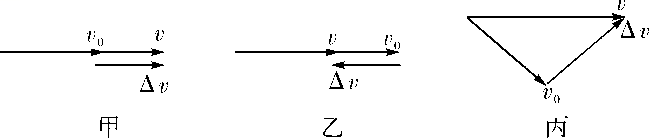
\includegraphics[width=0.8\textwidth]{11.png}
         \caption{速度变化量}
      \end{figure}

      \item 加速度
      \begin{itemize}
         \item 物理意义:描述物体速度变化快慢和变化方向的物理量,是状态量.
         \item 定义式:
         
         $a=\frac{\Delta v}{\Delta t}=\frac{v-v_{0}}{\Delta t}$.
         \item 决定因素:a不是由$v, \Delta t, \Delta v$来决定,而是由F、M来决定.
         \item 与$\Delta v$的方向一致,由合外力的方向决定,而与$v_{0}, v$的方向无关.
      \end{itemize}

   \end{enumerate}

   \section{对质点概念的理解}
   \begin{example}
      在研究下述运动时,能把物体看做质点的是( B )

      A.研究短跑运动员的起跑动作时

      B.研究一架无人机的飞行快慢时

      C.将一枚硬币用力上抛并猜测它落地时正面是朝上还是朝下时

      D.研究汽车在上坡时有无翻倒的危险时
      \begin{solution}
         研究短跑运动员的起跑动作、抛出硬币落地时的上下面时,所研究对象的大小和形状不能忽略,故运动员和硬币都不能看做质点;研究汽车翻倒是转动问题,不能将汽车看做质点;研究飞机飞行快慢时,可把飞机看做质点.故选项B正确.

         
      \end{solution}
      
   \end{example}
   \begin{note}
      建立质点模型的两个关键点
      \begin{itemize}
         \item 明确题目中要研究的问题是什么.
         
         质点是对实际物体的科学抽象,是研究物体运动时对实际物体进行的近似,真正的质点并不存在.
         \item 分析物体的大小和形状对所研究的问题产生的影响能否忽略不计.
         
         当物体的大小和形状对所研究运动的影响很小,可以忽略不计时,就可将其视为质点.
      \end{itemize}
   \end{note}


   \newpage\section{位移与路程的区别和联系}
      \begin{figure}[htbp]
         \centering
         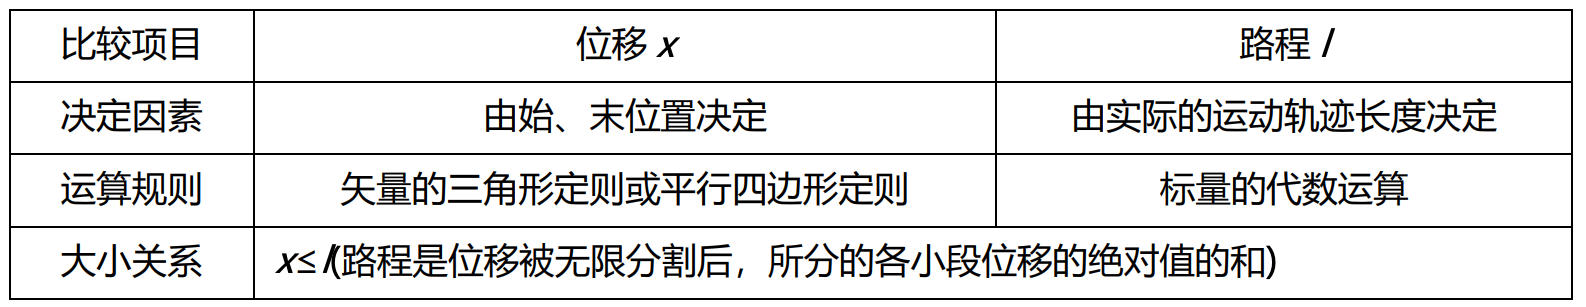
\includegraphics[width=0.8\textwidth]{t11.png}
      \end{figure}

      
      \begin{example}
         (2017·湖南株洲质检)(多选)关于位移和路程,下列说法正确的是( BD )

         A.物体在某一段时间内运动的位移为零,则其一定是静止的

         B.物体在某一段时间内运动的路程为零,则其一定是静止的

         C.在直线运动中,物体的位移大小一定等于其路程

         D.在曲线运动中,物体的位移大小一定小于路程
         \begin{solution}
            路程指物体运动轨迹的长度,而位移指由初位置指向末位置的有向线段,只有当物体做单向直线运动时,其位移大小才等于路程.容易判断选项B、D正确,A、C错误.

            
         \end{solution}

      
         
      \end{example}

   \newpage\section{平均速度与瞬时速度的区别和联系}
   \begin{itemize}
      \item 两种物体的速度
      \begin{itemize}
         \item 瞬时速度是运动时间$\Delta t \rightarrow 0$时的平均速度.
         \item 对于匀速直线运动,瞬时速度与平均速度相等.
      \end{itemize}
      \item 关于用平均速度法求瞬时速度
      \begin{itemize}
         \item 方法概述:由平均速度公式$\overline{v}=\frac{\Delta x}{\Delta t}$可知,当$\Delta x、\Delta t$都非常小,趋向于极限时,这时的平均速度就可认为是某一时刻或某一位置的瞬时速度.
         \item 选用思路:当已知物体在微小时间$\Delta t$内发生的微小位移$\Delta x$时,可由$\overline{v}=\frac{\Delta x}{\Delta t}$粗略地求出物体在该位置的瞬时速度.
            
      \end{itemize}
   \end{itemize}
   \begin{example}
      (多选)如图1.2所示,物体沿曲线轨迹的箭头方向运动,AB、ABC、ABCD、ABCDE四段曲线轨迹运动所用的时间分别是1 s、2 s、3 s、4 s.下列说法正确的是( ABC )
      \begin{figure}[htbp]
         \centering
         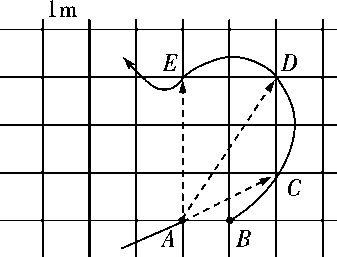
\includegraphics[width=0.2\textwidth]{12.png}
         \caption{}
      \end{figure}
   
      A.物体在AB段的平均速度大小为1 m/s
      
      B.物体在ABC段的平均速度大小为52 m/s
      
      C.AB段的平均速度比ABC段的平均速度更能反映物体处于A点时的瞬时速度
      
      D.物体在B点的速度等于AC段的平均速度
      \begin{solution}
         由$\overline{v}=\frac{\Delta x}{\Delta t}$可得$\overline{v}_{A B}=\frac{1}{1} \mathrm{m} / \mathrm{s}=1 \mathrm{m} / \mathrm{s}, \quad \overline{v}_{A C}=\frac{\sqrt{5}}{2} \mathrm{m} / \mathrm{s}$,故选项A、B均正确;所选取的过程离A点越近,其阶段的平均速度越接近A点的瞬时速度,故选项C正确;由A经B到C的过程不是匀变速直线运动过程,故B点虽为AC段的中间时刻,但其速度不等于AC段的平均速度,故选项D错误.
         
      \end{solution}
   
      
   \end{example}
   \begin{note}
      平均速度和瞬时速度的三点注意
      \begin{itemize}
         \item 求解平均速度必须明确是哪一段位移或哪一段时间内的平均速度.
         \item $\overline{v}=\frac{\Delta x}{\Delta t}$是平均速度的定义式,适用于所有的运动.
         \item 用平均速度法近似求解瞬时速度,不仅适用于直线运动,也适用于曲线运动.时间越短,平均速度越接近于瞬时速度.
      \end{itemize}
   \end{note}


   \newpage\section{速度、速度的变化量和加速度的关系}

   \begin{itemize}
      \item 速度的大小与加速度的大小没有必然联系.
      \item 速度变化量与加速度没有必然的联系,速度变化量的大小由加速度和速度变化的时间决定.
      \item $a=\frac{\Delta v}{\Delta t}$是加速度的定义式;加速度的决定式是$a=\frac{F}{m}$,即加速度的大小由物体受到的合力F和物体的质量m共同决定,加速度的方向由合力的方向决定.
      \item 速度增大或减小由速度与加速度的方向关系决定
      \begin{figure}[htbp]
         \centering
         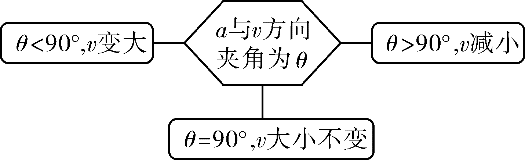
\includegraphics[width=0.4\textwidth]{13.png}
      \end{figure}
   
   \end{itemize}
   \begin{example}
      一质点在x轴上运动,初速度$v_{0}>0$,加速度$a>0$,当加速度a的值由零逐渐增大到某一值后再逐渐减小到零,则该质点( B )
      
      A.速度先增大后减小,直到加速度等于零为止
      
      B.速度一直在增大,直到加速度等于零为止
      
      C.位移先增大,后减小,直到加速度等于零为止
      
      D.位移一直在增大,直到加速度为0为止
      \begin{solution}
         由于加速度的方向始终与速度方向相同,质点速度逐渐增大,当加速度减小到零时,速度达到最大值,选项A错误,B正确;位移逐渐增大,当加速度减小到零时,速度不再变化,位移将随时间继续增大,选项C、D错误.

         
      \end{solution}
   
      
   \end{example}
   \begin{note}
      对加速度大小和方向的进一步理解
      \begin{figure}[htbp]
         \centering
         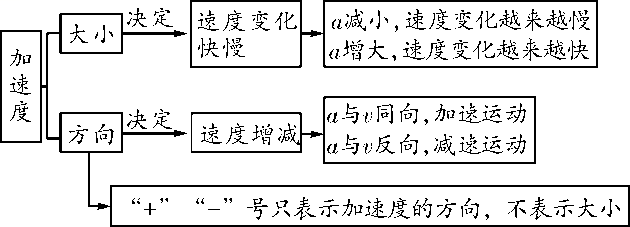
\includegraphics[width=0.5\textwidth]{14.png}
      \end{figure}

      
   \end{note}

   

\chapter{匀变速直线运动的规律及应用}
\begin{enumerate}
   \item 基本规律
   \begin{itemize}
      \item 速度公式:$v=v_{0}+a t$
      \item 位移公式:$x=v_{0} t+\frac{1}{2} a t^2$
      \item 位移速度关系式:$v^{2}-v_{0}^{2}=2 a x$
   \end{itemize}
   \item 两个重要推论
   \begin{itemize}
      \item 物体在一段时间内的平均速度等于这段时间中间时刻的瞬时速度,还等于初、末时刻速度矢量和的一半,即
      
      $v_{\frac{t}{2}}=\frac{v_{0}+v}{2}$..
      \item 任意两个连续相等的时间间隔T内的位移之差为一恒量,即
      
      $\Delta x=x_{2}-x_{1}=x_{3}-x_{2}=\ldots=x_{n}-x_{n-1}=a T^{2}$
   \end{itemize}
   \item $v_{0}=0$的四个重要推论
   \begin{itemize}
      \item 1T末、2T末、3T末……瞬时速度的比为
      
      $v_{1} : v_{2} : v_{3} : \ldots : v_{n}=1 : 2 : 3 : \ldots : n$..
      \item 1T内、2T内、3T内……位移的比为
      
      $x_{1} : x_{2} : x_{3} : \ldots : x_{0}=1^{2} : 2^{2} : 3^{2} : \ldots : n^{2}$.
      \item 第一个T内、第二个T内、第三个T内……位移的比为
      
      $x_{\mathrm{I}} : x_{\mathrm{II}} : x_{\mathrm{III}} : \ldots : x_{n}=1 : 3 : 5 : \ldots :(2 n-1)$.
      \item 从静止开始通过连续相等的位移所用时间的比为
      
      $t_{1} : t_{2} : t_{3} : \ldots : t_{n}=1 :(\sqrt{2}-1) :(\sqrt{3}-\sqrt{2}) : \ldots :(\sqrt{n}-\sqrt{n-1})$.  
   \end{itemize}
   \item 自由落体运动
   \begin{itemize}
      \item 条件:物体只受重力,从静止开始下落..
      \item 基本规律:
      \begin{itemize}
         \item 速度公式$v=g t$;
         \item 位移公式$h=\frac{1}{2} g t^{2}$;
         \item 速度位移关系式$v^{2}=2 g h$.
      \end{itemize}
   \end{itemize}
   \item 竖直上抛运动
   \begin{itemize}
      \item 运动特点:
      
      加速度为g,上升阶段做匀减速直线运动,下降阶段做自由落体运动.
      \item 基本规律:
      \begin{itemize}
         \item 速度公式$v=v_{0}-g t$;
         \item 位移公式$h=v_{0} t-\frac{1}{2} g t^{2}$;
         \item 速度位移关系式$v^{2}-v_{0}^{2}=-2 g h$.
      \end{itemize}
   \end{itemize}
\end{enumerate}

   \section{匀变速直线运动的规律及应用}
   \begin{itemize}
      \item 运动学公式中正、负号的规定
      \begin{itemize}
         \item 除时间$t$外,$x, v_{0}, v, a$均为矢量,所以需要确定正方向,一般以$v_{0}$的方向为正方向.
         与初速度同向的物理量取正值,反向的物理量取负值,当$v_{0}=0$时,一般以加速度a的方向为正方向.
         \item 五个物理量$t, v_{0},  v,  a, x$必须针对同一过程.
      \end{itemize}
      \item 解决匀变速直线运动问题常用的“六法”
      
      \begin{figure}[htbp]
         \centering
         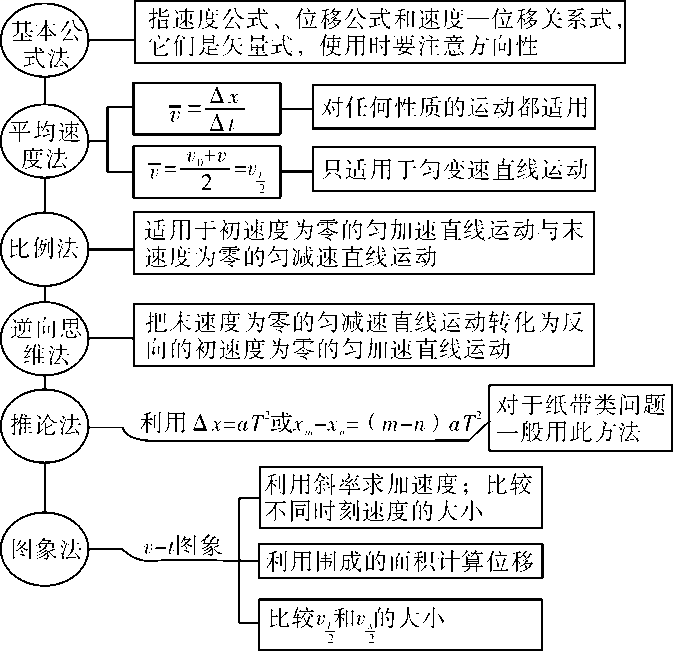
\includegraphics[width=0.5\textwidth]{15.png}
      \end{figure}

      \begin{example}
         (2017·湖南岳阳检测)如图所示,是冰壶以速度v垂直进入四个宽为l的矩形区域沿虚线做匀减速直线运动,且刚要离开第四个矩形区域的E点时速度恰好为零,冰壶通过前三个矩形的时间为t,试通过所学知识分析并计算冰壶通过第四个矩形所用的时间是多少?(可选用多种方法)
      
      \begin{figure}[htbp]
         \centering
         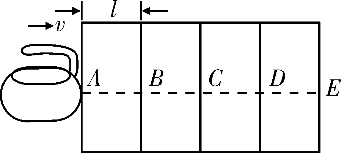
\includegraphics[width=0.2\textwidth]{16.png}
      \end{figure}
      
         \begin{solution}

            根据位移公式和速度公式,由A到E,有
            $4 l=v t_{1}-\frac{1}{2} a t^{2}, \quad 0=v-a t_{1}$,
            式中,$t_{1}$为冰壶通过四个矩形区域所用的时间,a为其加速度的大小,
            由A到D,有$3 l=v t-\frac{1}{2} a t^{2}$,
            联立解得$t_{1}=2 t$或$t_{1}=\frac{2}{3} t$,
            显然$t_{1}=\frac{2}{3} t$不符合题意,应舍去.
            所以冰壶通过第四个矩形所用的时间为$t^{\prime}=t_{1}-t=t$.

            答案  t

            
         \end{solution}   
         
      \end{example}
      \begin{note}
         求解匀变速直线运动问题的基本思路
               
      \begin{figure}[htbp]
         \centering
         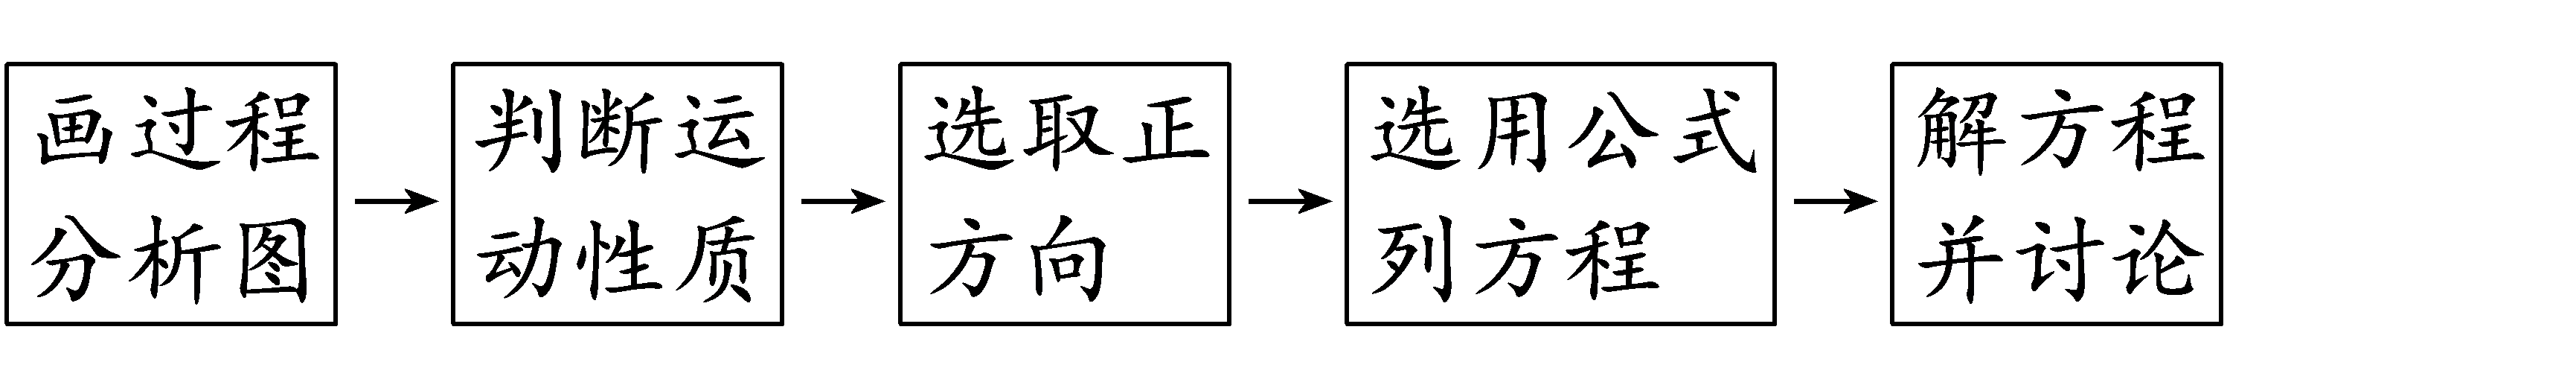
\includegraphics[width=0.5\textwidth]{17.png}
      \end{figure}
      

      \end{note}
   \end{itemize}

   \section{自由落体和竖直上抛运动的分析}
   \begin{example}
      (2017·山东济南调研)如图所示是一种较精确测量重力加速度g值的方法:将下端装有弹射装置的真空玻璃直管竖直放置,玻璃管足够长,小球竖直向上被弹出,在O点与弹簧分离,然后返回,在O点正上方选取一点P,利用仪器精确测得OP间的距离为H,从O点出发至返回O点的时间间隔为T1,小球两次经过P点的时间间隔为T2.求:
      
      (1)重力加速度g;
      
      (2)若O点距玻璃管底部的距离为L0,求玻璃管最小长度.
   \begin{solution}
      (1)小球从O点上升到最高点有$h_{1}=\frac{1}{2} g\left(\frac{T_{1}}{2}\right)^{2}$
      ,小球从P点上升到最高点有$h_{2}=\frac{1}{2} g\left(\frac{T_{2}}{2}\right)$
      ,依据题意有$h_{1}-h_{2}=H$,联立解得$g=\frac{8 H}{T_{1}^{2}-T_{2}^{2}}$.
      
      (2)真空管最小长度$L=L_{0}+h_{1}$,解得$L=L_{0}+\frac{T_{1}^{2} H}{T_{1}^{2}-T_{2}^{2}}$.
      
      答案 

      (1)$\frac{8 H}{T_{1}^{2}-T_{2}^{2}}$ 
      
      (2)$L_{0}+\frac{T_{1}^{2} H}{T_{1}^{2}-T_{2}^{2}}$
   \end{solution}   
   \end{example}
   \begin{note}
      竖直上抛运动的分析方法
      \begin{itemize}
         \item 分段法:可以把竖直上抛运动分成上升阶段的匀减速运动和下降阶段的自由落体运动处理,下降过程是上升过程的逆过程.
         \item 整体法:从全过程来看,加速度方向始终与初速度的方向相反,所以也把竖直上抛运动看成是一个匀变速直线运动.
      \end{itemize}
      
   \end{note}

   

\chapter{运动图象追及和相遇问题}
\begin{enumerate}
   \item 直线运动的x-t图象
   \begin{itemize}
      \item 意义:反映了直线运动的物体位移随时间变化的规律.
      \item 图线上某点切线的斜率的意义
      \begin{itemize}
         \item 斜率大小:表示物体速度的大小
         \item 斜率的正负:表示物体速度的方向
      \end{itemize}
      \item 两种特殊的x-t图象
      \begin{itemize}
         \item 若x-t图象是一条平行于时间轴的直线,说明物体处于静止状态. (如图所示甲图线)
         \item 若x-t图象是一条倾斜的直线,说明物体在做匀速直线运动. (如图所示乙图线)
      \end{itemize}
   \end{itemize}
   \item 直线运动的v-t图象
   \begin{itemize}
      \item 意义:反映了直线运动的物体速度随时间变化的规律.
      \item 图线上某点切线的斜率的意义.
      \begin{itemize}
         \item 斜率的大小:表示物体加速度的大小
         \item 斜率的正负:表示物体加速度的方向
      \end{itemize}
      \item 两种特殊的v-t图象
      \begin{itemize}
         \item 匀速直线运动的v-t图象是与横轴平行的直线. (如图所示甲图线)
         \item 匀变速直线运动的v-t图象是一条倾斜的直线. (如图所示乙图线)
      \end{itemize}
      \item 图线与坐标轴围成的“面积”的意义
      \begin{itemize}
         \item 图线与坐标轴围成的“面积”表示相应时间内的位移.
         \item 若此面积在时间轴的上方,表示这段时间内的位移方向为正方向;若此面积在时间轴的下方,表示这段时间内的位移方向为负方向.
      \end{itemize}
   \end{itemize}
   \item 追及和相遇问题
   \begin{itemize}
      \item 两类追及问题.
      \begin{itemize}
         \item 若后者能追上前者,追上时,两者处于同一位置,且后者速度一定不小于前者速度.
         \item 若追不上前者,则当后者速度与前者相等时,两者相距最近            
      \end{itemize}
      \item 两类相遇问题
      \begin{itemize}
         \item 同向运动的两物体追及,追上时即相遇
         \item 相向运动的物体,当各自发生的位移大小之和等于开始时两物体间的距离时即相遇
         
      \end{itemize}
   \end{itemize}
\end{enumerate}

   \section{x-t图象与v-t图象的区别}
   \begin{figure}[htbp]
      \centering
      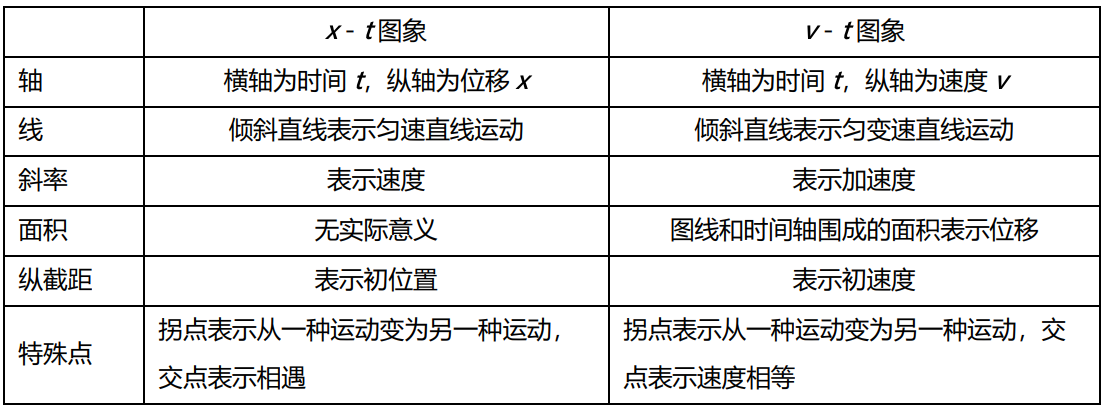
\includegraphics[width=1\textwidth]{t12.png}
   \end{figure}
   \begin{example}
      (2018·陕西汉中期末)在平直的公路上行驶的a车和b车,其位移—时间图象分别为图中直线a和曲线b,已知b车的加速度恒定且ab=-2 m/s2,当t=3 s时,直线a和曲线b刚好相切,求t=0 s时a车和b车的距离x0.      

      \begin{figure}[htbp]
      \centering
      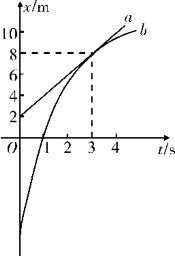
\includegraphics[width=0.2\textwidth]{19.png}
   \end{figure}

      \begin{solution}
         答案 9 m
         
      \end{solution}   
      
   \end{example}
   \begin{note}
      运动图象中的易错点
      \begin{itemize}
         \item 对x-t图象,图线在纵轴上的截距表示t=0时物体的位置,对v-t或a-t图象,图线在纵轴上的截距并不表示t=0时物体的位置.
         \item 在v-t图象中,两条图线的交点不表示两物体相遇,而是表示两者速度相同.
         \item 两条图线在v轴上的截距不同,不少同学误认为两物体的初始位置不同,位置是否相同应根据题中条件确定.
      \end{itemize}
      
   \end{note}

   \newpage\section{追及、相遇问题}
   讨论追及、相遇的问题,其实质就是分析讨论两物体在同一时刻能否到达相同的空间位置问题.
   \begin{itemize}
      \item 抓住一个条件,两个关系
      \begin{itemize}
         \item 一个条件:即两者速度相等,它往往是物体间能否追上、追不上或(两者)距离最大、最小的临界条件,也是分析判断的切入点.
         \item 两个关系:即时间关系和位移关系,这两个关系可通过画运动示意图得到.
      \end{itemize}
      \item 能否追上的判断方法
      
      常见情形:物体A追物体B,开始二者相距$x_{0}$,则
      \begin{itemize}
         \item A追上B时,必有$x_{A}-x_{B}=x_{0}$,且$v_{A} \geq v_{B}$.
         \begin{figure}[htbp]
            \centering
            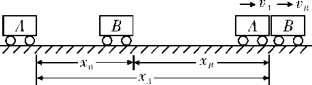
\includegraphics[width=0.5\textwidth]{110.png}
         \end{figure}

         \item 要使两物体恰好不相撞,必有xA-xB=x0,vA=vB.
      \end{itemize}
      
   \end{itemize}
   \begin{example}
      (2018·江苏镇江模拟)甲、乙两车在同一直线轨道上同向行驶,
      甲车在前,速度为$v_{1}=8 \mathrm{m} / \mathrm{s}$,乙车在后,速度为$v_{2}=16m/s$,
      当两车相距$x_{0}=8 \mathrm{m}$时,甲车因故开始刹车,
      加速度大小为$a_{1}=2 \mathrm{m} / \mathrm{s}^{2}$,为避免相撞,
      乙车立即开始刹车,则乙车的加速度至少为多大?         

      \begin{solution}

         答案 6 $\mathrm{m} / \mathrm{s}^{2}$               
      \end{solution}   
      
   \end{example}

   \begin{note}
      追及和相遇问题的求解方法
      \begin{itemize}
         \item 解题思路
         \begin{figure}[htbp]
            \centering
            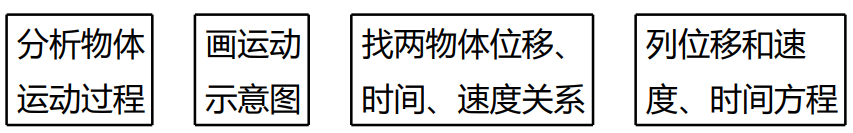
\includegraphics[width=0.5\textwidth]{111.png}
         \end{figure}

         \item 解题技巧
         \begin{itemize}
            \item 紧抓“一图三式”,即:过程示意图,时间关系式、速度关系式和位移关系式.
            \item 审题应抓住题目中的关键字眼,充分挖掘题目中的隐含条件.如“刚好”“恰好”“最多”“至少”等.往往对应一个临界状态,满足相应的临界条件.
            \item 若被追赶的物体做匀减速运动,一定要注意追上前该物体是否已经停止运动,另外还要注意最后对解的讨论分析.
         \end{itemize}
      \end{itemize}
      
   \end{note}



\chapter{重力 弹力 摩擦力}
   \begin{enumerate}
      \item 重力
      \begin{itemize}
         \item 产生:由于地球的吸引而使物体受到的力
         \item 大小:与物体的质量成正比,即$G=m g$.可用弹簧测力计测量重力.
         \item 方向:总是竖直向下的
         \item 重心:其位置与物体的质量分布和形状有关
         
      \end{itemize}
      \item 弹力
      \begin{itemize}
         \item 定义:发生弹性形变的物体由于要恢复原状而对与它接触的物体产生的作用力
         \item 产生的条件
         \begin{itemize}
            \item 物体间直接接触;
            \item 接触处发生弹性形变
            
         \end{itemize}
         \item 方向:总是与物体形变的方向相反
         
      \end{itemize}
      \item 胡克定律
      \begin{itemize}
         \item 内容:在弹性限度内,弹力的大小跟弹簧伸长(或缩短)的长度x成正比.
         \item 表达式:$F=k x$.$k$是弹簧的劲度系数,由弹簧自身的性质决定,单位是牛顿每米,用符号$\mathrm{N} / \mathrm{m}$表示. $x$是弹簧长度的变化量,不是弹簧形变以后的长度.
         
      \end{itemize}
      \item 滑动摩擦力和静摩擦力的对比
      \begin{figure}[htbp]
         \centering
         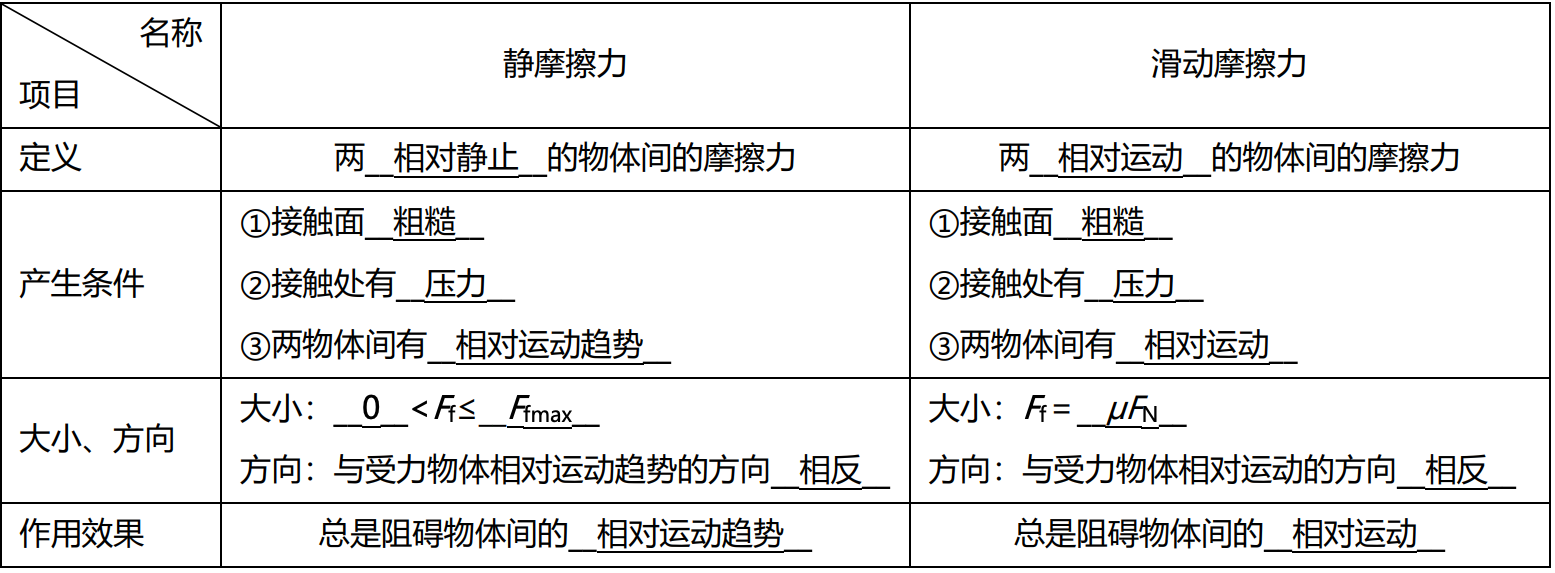
\includegraphics[width=1\textwidth]{t14.png}
      \end{figure}
      
      滑动摩擦力大小的计算公式$F_{\mathrm{f}}=\mu F_{\mathrm{N}}$中$μ$为比例常数,称为动摩擦因数,其大小与两个物体的材料和接触面的粗糙程度有关.
   \end{enumerate}

   \newpage\section{弹力有无的判断}
   \begin{figure}[htbp]
      \centering
      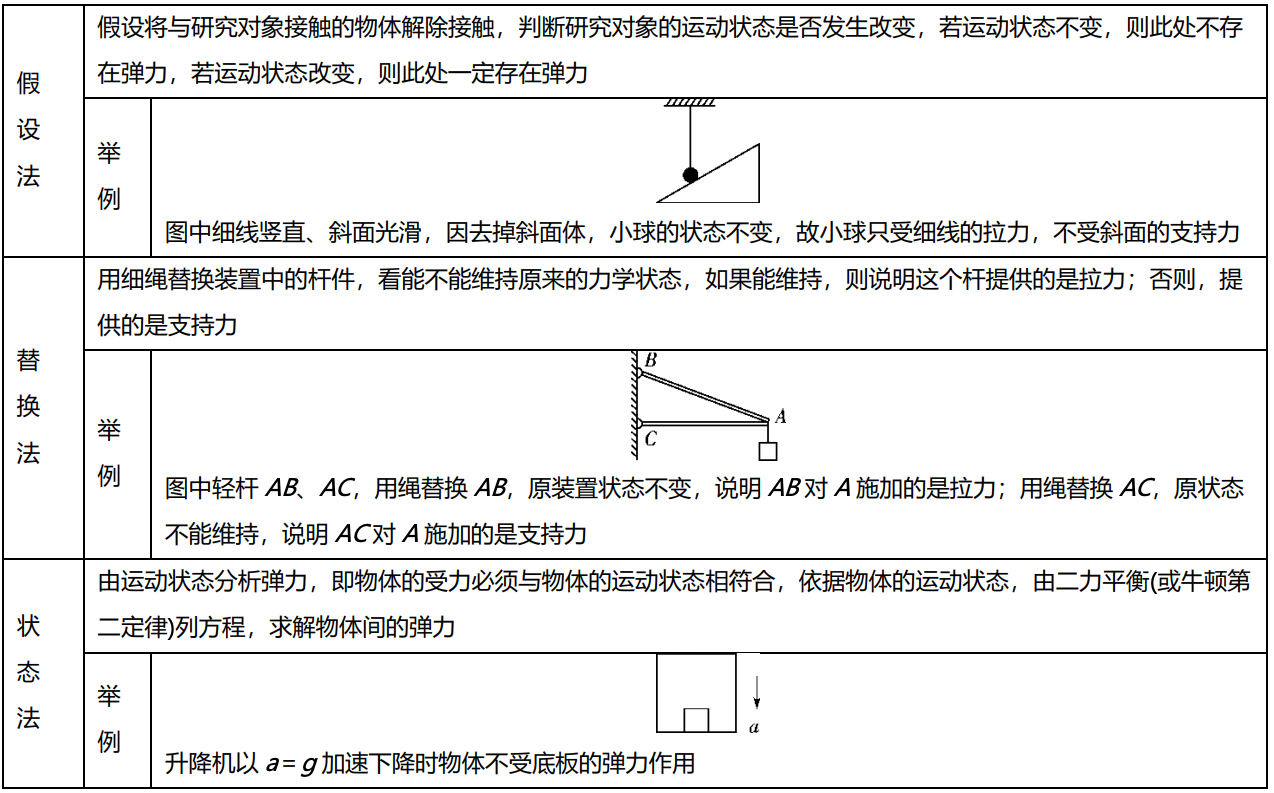
\includegraphics[width=1\textwidth]{t13.png}
   \end{figure}

   \begin{example}
      (2017·陕西西安调研)如图所示,在一个正方体的盒子中放有一个质量
      分布均匀的小球,小球的直径恰好和盒子内表面正方体的棱长相等,
      盒子沿倾角为α的固定斜面滑动,不计一切摩擦,
      下列说法中正确的是( A )         
      \begin{figure}[htbp]
      \centering
      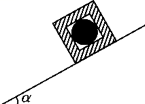
\includegraphics[width=0.3\textwidth]{21.png}
   \end{figure}
   
      \begin{solution}
         先以盒子和小球组成的系统为研究对象,无论上滑还是下滑,
         用牛顿第二定律均可求得系统的加速度大小为$a=g \sin \alpha$,
         方向沿斜面向下,由于盒子和小球始终保持相对静止,
         所以小球的加速度大小也是$a=g \sin \alpha$,方向沿斜面向下,
         小球沿斜面向下的重力分力大小恰好等于所需的合外力,
         因此不需要盒子的左、右侧面提供弹力.故选项A正确.               
      \end{solution}   
      
   \end{example}
   \begin{note}
      对于形变明显的物体,由形变情况直接判断弹力情况,对于形变不明显的物体通常用“假设法”和“替换法”,有时要根据物体的运动状态判定弹力情况.

      
   \end{note}

   \newpage\section{弹力方向的确定和大小的计算}
   \begin{itemize}
      \item 弹力方向的确定
      \begin{figure}[htbp]
         \centering
         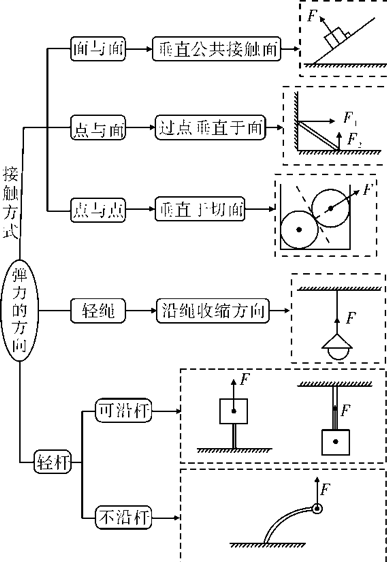
\includegraphics[width=0.6\textwidth]{t15.png}
      \end{figure}

      \item 计算弹力大小的三种方法
      \begin{itemize}
         \item 根据胡克定律进行求解
         \item 根据力的平衡条件进行求解
         \item 根据牛顿第二定律进行求解
      \end{itemize}

   \end{itemize}

   \newpage

   \begin{example}
      如图所示,固定在小车支架上的斜杆与竖直杆的夹角为θ,
      在斜杆下端固定一个质量为m的小球,
      下列关于杆对球的作用力F的判断中正确的是( D )    
      
      A.小车静止时,$F=m g \cos \theta$,方向沿杆向上
      
      B.小车静止时,$F=m g \cos \theta$,方向垂直杆向上

      C.小车向右以加速度a运动时,一定有$F=\frac{m g}{\sin \theta}$

      D.小车向左以加速度a运动时,$F=\sqrt{(m a)^{2}+(m g)^{2}}$,
      方向斜向左上方,与竖直方向的夹角为α满足$\tan \alpha=\frac{a}{g}$

      \begin{figure}[htbp]
         \centering
         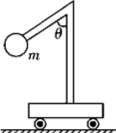
\includegraphics[width=0.3\textwidth]{112.png}
      \end{figure}
   
      \begin{solution}
         先以盒子和小球组成的系统为研究对象,无论上滑还是下滑,
         用牛顿第二定律均可求得系统的加速度大小为$a=g \sin \alpha$,
         方向沿斜面向下,由于盒子和小球始终保持相对静止,
         所以小球的加速度大小也是$a=g \sin \alpha$,方向沿斜面向下,
         小球沿斜面向下的重力分力大小恰好等于所需的合外力,
         因此不需要盒子的左、右侧面提供弹力.故选项A正确.               
      \end{solution}   
      
   \end{example}

   \begin{example}
      缓冲装置可抽象成如图所示的简单模型,图中A、B为原长相等、
      劲度系数分别为$k_{1}, k_{2}\left(k_{1} \neq k_{2}\right)$的两个不同的轻质弹簧.
      下列表述正确的是( D )
      \begin{figure}[htbp]
         \centering
         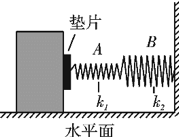
\includegraphics[width=0.2\textwidth]{113.png}
      \end{figure}
   
      A.装置的缓冲效果与两弹簧的劲度系数无关

      B.垫片向右移动稳定后,两弹簧产生的弹力之比$F_{1} : F_{2}=k_{1} : k_{2}$ 

      C.垫片向右移动稳定后,两弹簧的长度之比$I_{1} : l_{2}=k_{2} : k_{1}$

      D.垫片向右移动稳定后,两弹簧的压缩量之比$x_{1} : x_{2}=k_{2} : k_{1}$ 

      
   \end{example}

   \newpage\section{静摩擦力的大小和方向}
   \begin{itemize}
      \item 静摩擦力有无的判断
      \begin{itemize}
         \item 假设法
         静摩擦力的方向一定与物体相对运动趋势的方向相反,利用“假设法”可以判断出物体相对运动趋势的方向.
         假设法(如图所示)
                        
         \begin{figure}[htbp]
            \centering
            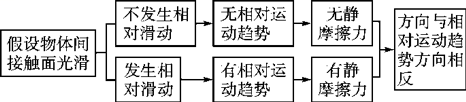
\includegraphics[width=0.3\textwidth]{t16.png}
         \end{figure}

         \item 状态法
         
         此法关键是先判明物体的运动状态(即加速度的方向),再利用牛顿第二定律(F=ma)确定合力,
         然后通过受力分析确定静摩擦力的大小及方向.
         \item 牛顿第三定律法
         
         此法的关键是抓住“力是物体间的相互作用”,
         先确定受力较少的物体受到的静摩擦力的方向,
         再根据“力的相互性”确定另一物体受到的静摩擦力方向.
      \end{itemize}
      \item 静摩擦力的计算方法
      \begin{itemize}
         \item 最大静摩擦力$F_{\mathrm{fmax}}$的计算
         最大静摩擦力$F_{\mathrm{fmax}}$只在刚好要发生相对滑动这一特定状态下才表现出来.
         比滑动摩擦力稍大些,
         通常认为二者相等,即$F_{\max }=\mu F_{N}$. 
         \item 一般静摩擦力的计算
         一般静摩擦力F的大小和方向都与产生相对运动趋势的力密切相关,
         跟接触面间相互挤压的弹力$F_{\mathrm{N}}$无直接关系,因此具有大小、方向的可变性.对具体问题要结合研究对象的运动状态(静止、匀速运动或加速运动),
         利用平衡条件或牛顿运动定律列方程求解.
      \end{itemize}
   \end{itemize}
   \begin{example}
      (2018·宁夏银川检测)指明物体A在以下四种情况下所受的静摩擦力的方向.
      \begin{figure}[htbp]
         \centering
         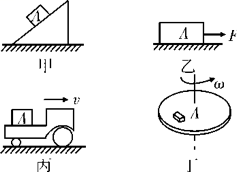
\includegraphics[width=0.2\textwidth]{114.png}
      \end{figure}
   
      (1)物体A静止于斜面上,如图甲所示;

      (2)物体A受到水平拉力F作用而仍静止在水平面上,如图乙所示;

      (3)物体A放在车上,在刹车过程中A相对于车厢静止,如图丙所示;

      (4)物体A在水平转台上,随转台一起匀速运动,如图丁所示.
      
      
   \end{example}
   \begin{note}
      应用“状态法”解题时应注意的问题

      状态法是分析判断静摩擦力有无及方向、大小的常用方法,在使用状态法处理问题时,需注意以下两点:
      \begin{itemize}
         \item 明确物体的运动状态,分析物体的受力情况,根据平衡方程或牛顿定律求解静摩擦力的大小和方向.
         \item 静摩擦力的方向与物体的运动方向没有必然关系,可能相同,也可能相反,还可能成一定的夹角.
      \end{itemize}
      
   \end{note}

   \section{滑动摩擦力的大小和方向}
   \begin{itemize}
      \item 产生的条件
      \begin{itemize}
         \item 两物体相互接触且挤压,发生形变,产生弹力.
         \item 两接触面粗糙.
         \item 两物体沿接触面发生相对运动.
         
         以上三个条件必须同时具备,才会有滑动摩擦力存在.
      \end{itemize}
      \item 在计算滑动摩擦力的公式$F_{f}=\mu F_{N}$中,μ为动摩擦因数,
      其大小与接触面的材料、表面的粗糙程度有关;$F_{\mathrm{N}}$为两接触面间的正压力,其大小不一定等于物体的重力.
      \item 滑动摩擦力的大小与物体的运动速度无关,与接触面积也无关.
      \item 滑动摩擦力的方向总是与物体间相对运动的方向相反,但不一定与物体运动方向相反.

   \end{itemize}

   \begin{example}
      (2017·吉林长春检测)如图所示,质量为m的工件置于水平放置的钢板C上,
      二者间动摩擦因数为μ,由于固定的光滑导槽A、B的控制,工件只能沿水平导槽运动,
      现使钢板以速度$v_{1}$向右运动,
      同时用F拉动工件(F方向与导槽平行)使其以速度$v_{2}$沿导槽运动,则F的大小为( C )  
      \begin{figure}[htbp]
         \centering
         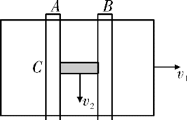
\includegraphics[width=0.2\textwidth]{115.png}
      \end{figure}
   
      A.等于μmg	
      
      B.大于μmg

      C.小于μmg	
      
      D.不能确定

      \begin{solution}
         钢板以速度$v_{1}$向右运动,则工件以等大速度相对钢板向左移动,设为$v_{1}$,
         同时工件被拉动也具有另一速度$v_{2}$,
         故工件相对于钢板的运动速度应是$v_{1}$与$v_{2}$的合成,即如上图中的速度v.滑动摩擦力阻碍二者的相对运动,故工件所受摩擦力Ff与v方向相反,
         要使工件沿导槽匀速运动,所施加的拉力只需与$F_{f}$一个分力平衡,
         故$F<F_{f} = μmg$.
         \begin{figure}[htbp]
            \centering
            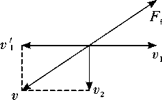
\includegraphics[width=0.2\textwidth]{116.png}
         \end{figure}

      \end{solution}
                  
      
   \end{example}

   \newpage\section{摩擦力突变问题}
   \begin{note}
      解决摩擦力突变问题的关键点

      物体受到的外力发生变化时,
      物体受到的摩擦力的种类就有可能发生突变.
      解决这类问题的关键是:正确对物体受力分析和运动状态分析,
      从而找到物体摩擦力的突变“临界点”.
      
      常见类型如下:

      \begin{itemize}
         \item 静—静“突变”
         
         当作用在物体上的其他力的合力发生变化时,
         物体仍保持静止,而所受静摩擦力方向发生180°“突变”,则“突变”点是静摩擦力为零时.
         \item 动—动“突变”
         
         某物体相对于另一物体滑动的过程中,若相对运动方向变了,
         则滑动摩擦力方向发生“突变”,“突变”点为两物体相对速度为零时.
         \item 静—动“突变”
         
         物体在摩擦力和其他力作用下处于静止状态,当其他力变化时,如果物体不能保持静止状态,
         则物体受到的静摩擦力将“突变”成滑动摩擦力,“突变”点为静摩擦力达到最大值时.
         \item 动—静“突变”
         
         两物体相对减速滑动的过程中,若相对速度变为零,
         则滑动摩擦力“突变”为静摩擦力,“突变”点为两物体相对速度刚好为零时.
      \end{itemize}
      
   \end{note}

   \begin{example}
      (多选)如图所示,将两相同的木块a、b置于粗糙的水平地面上,
      中间用一轻弹簧连接,两侧用细绳系于墙壁.开始时a、b均静止,弹簧处于伸长状态,
      两细绳均有拉力,a所受摩擦力Ffa≠0,b所受摩擦力Ffb=0.
      现将右侧细绳剪断,则剪断瞬间( AD )   

      \begin{figure}[h]
         \centering
         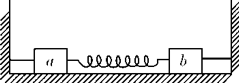
\includegraphics[width=0.2\textwidth]{117.png}
      \end{figure}
   
      A.Ffa大小不变	
      
      B.Ffa方向改变

      C.Ffb仍然为零	
      
      D.Ffb方向向右
      
                  
      
   \end{example}

   \newpage

   \begin{example}
      传送带以恒定的速率v=10 m/s运动,
      已知它与水平面成α=37°,如图所示,PQ=16 m,
      将一个小物体无初速度地放在P点,小物体与传送带间的动摩擦因数为μ=0.5,
      问当传送带逆时针转动时,
      小物体运动到Q点的时间为多少?
      (cos 37°=0.8,sin 37°=0.6,g取10 m/s2)

      \begin{figure}[htbp]
         \centering
         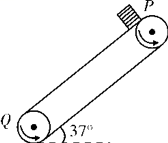
\includegraphics[width=0.5\textwidth]{118.png}
      \end{figure}
   
      \begin{solution}
         答案 2 s   
      \end{solution}
                  
      
   \end{example}

   \begin{note}
      摩擦力突变问题的分析步骤
      \begin{figure}[h]
         \centering
         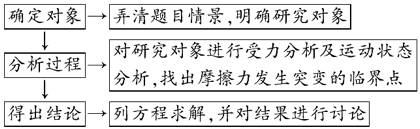
\includegraphics[width=0.6\textwidth]{t17.png}
      \end{figure}

      
   \end{note}



\chapter{力的合成与分解}
   \begin{enumerate}
      \item 力的合成
      \begin{itemize}
         \item 合力与分力
         \begin{itemize}
            \item 定义:如果几个力共同作用产生的效果与一个力的作用效果相同,这一个力就叫做那几个力的合力,那几个力叫做这一个力的分力
            \item 关系:合力与分力是等效替代关系
            
         \end{itemize}
         \item 共点力:作用在物体的同一点,或作用线的延长线交于一点的几个力
         \item 力的合成
         \begin{itemize}
            \item 定义:求几个力的合力的过程
            \item 运算法则
            \begin{itemize}
               \item 平行四边形定则:求两个互成角度的共点力的合力,可以用表示这两个力的线段为邻边作平行四边形,这两个邻边之间的对角线就表示合力的大小和方向(图甲).
               \item 三角形定则:把两个矢量的首尾顺次连接起来,第一个矢量的首到第二个矢量的尾的有向线段为合矢量(图乙).
               
            \end{itemize}
            
         \end{itemize}
         
      \end{itemize}
      \item 力的分解
      \begin{itemize}
         \item 定义:求一个力的分力的过程,力的分解是力的合成的逆运算
         \item 遵循的原则
         \begin{itemize}
            \item 平行四边形定则
            \item 三角形定则
            
         \end{itemize}
         \item 分解方法
         \begin{itemize}
            \item 力的作用效果分解法
            \item 正交分解法
            
         \end{itemize}
         
      \end{itemize}
      \item 矢量和标量
      \begin{itemize}
         \item 矢量
         
         既有大小又有方向的物理量,相加时遵循平行四边形定则. 如速度、力等.
            
         \item 标量
         
         只有大小没有方向的物理量,求和时按算术法则相加. 如路程、动能等.
      \end{itemize}
      
   \end{enumerate}

   \newpage\section{共点力合成的常用方法}
   \begin{itemize}
      \item 共点力合成的常用方法
      \begin{itemize}
         \item 作图法
         
         从力的作用点沿两个分力的作用方向按同一标度作出两个分力F1、F2,
         以这两个力为邻边作一个平行四边形,这两个力所夹对角线表示这两个力的合力.
         通常可分别用刻度尺和量角器直接量出合力的大小和方向.
         \item 解析法
         
         根据力的平行四边形定则作出力的合成的图示,如图所示.
         \begin{figure}[h]
            \centering
            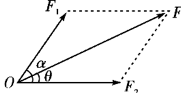
\includegraphics[width=0.2\textwidth]{511.png}
         \end{figure}
         F=F21+F22+2F1F2cos  α.
         它与F2的夹角为θ,tan  θ=F1sin  αF2+F1cos  α.

   
      \end{itemize}
      \item 几种特殊情况的共点力的合成
      \begin{figure}[h]
         \centering
         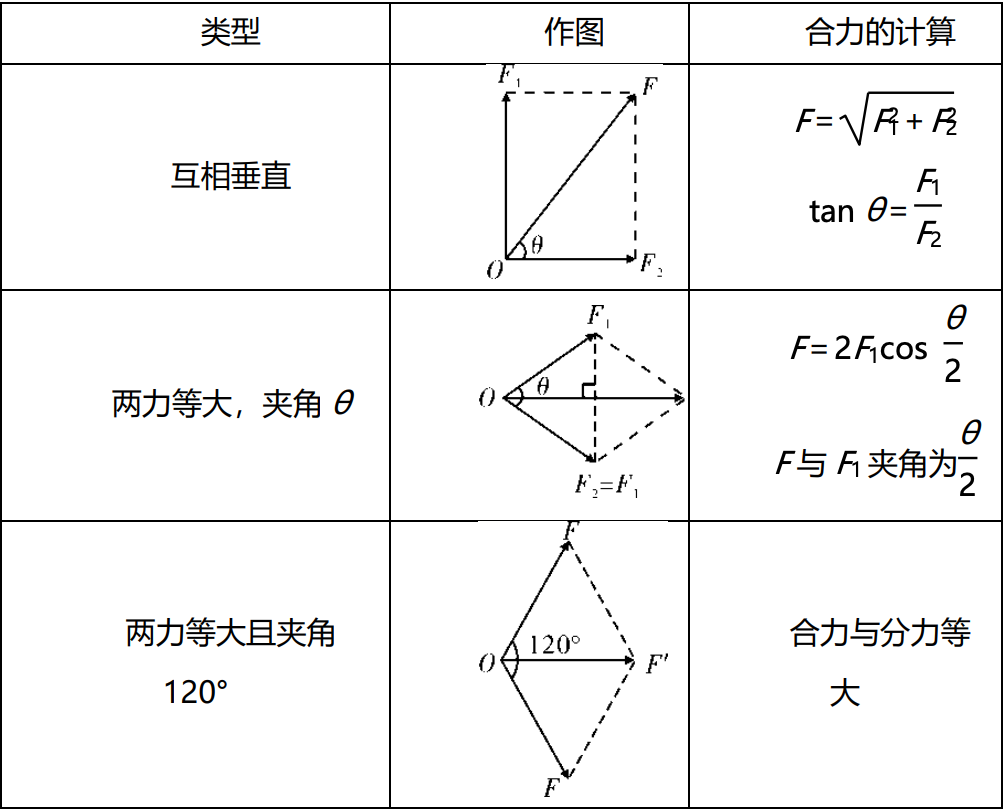
\includegraphics[width=0.6\textwidth]{512.png}
      \end{figure}

   \end{itemize}
   \begin{note}
      作图法求合力的四点要求
      \begin{itemize}
         \item 分力、合力的作用点相同,切忌弄错表示合力的对角线
         \item 分力、合力的比例要一致,力的标度要适当
         \item 虚线、实线要分清,表示分力和合力的两条邻边和对角线画成实线,
         并加上箭头,平行四边形的另两条边画成虚线
         \item 求合力时既要求出合力的大小,又要求出合力的方向
      \end{itemize}
      
   \end{note}

   \newpage

   \begin{example}
      (2017·天津卷)(多选)如图所示,
      轻质不可伸长的晾衣绳两端分别固定在竖直杆 M、N 上的 a、b 两点,
      悬挂衣服的衣架挂钩是光滑的,
      挂于绳上处于静止状态.如果只人为改变一个条件,
      当衣架静止时,下列说法正确的是( AB )
      \begin{figure}[htbp]
         \centering
         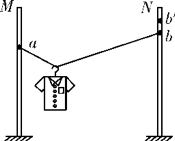
\includegraphics[width=0.3\textwidth]{513.png}
      \end{figure}
   
      \begin{solution}
      oa、ob为一根绳,两端拉力相等,设绳aob长为L,
      M、N的水平距离为d,bo延长线交M于a′,
      由几何知识知a′o=ao,sin θ=dL,
      由平衡条件有2Fcos θ=mg,则F=mg2cos θ,
      当b上移到b′时,d、L不变,θ不变,故F不变,
      选项A正确,C错误.将杆N向右移一些,L不变,d变大,θ变大,cos θ变小,
      则F变大,选项B正确.只改变m,其他条件不变,
      则sin θ不变,θ不变,衣架悬挂点不变,选项D错误. 
      \begin{figure}[htbp]
         \centering
         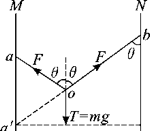
\includegraphics[width=0.3\textwidth]{514.png}
      \end{figure}
     
      \end{solution}
                  
      
   \end{example}

   \begin{note}
      \begin{itemize}
         \item 力合成时,要正确理解合力与分力的大小关系:
         合力与分力的大小关系要视情况而定,不能形成合力总大于分力的思维定式.
         \item 合力与它的分力是等效替代关系,
         在进行有关力的计算时,如果已计入了合力,就不能再计入分力;
         如果已计入了分力,就不能再计入合力.
      \end{itemize}
      
   \end{note}

   \newpage\section{力的分解}

   \begin{itemize}
      \item 按力的作用效果分解(思路图)
      \begin{figure}[htbp]
         \centering
         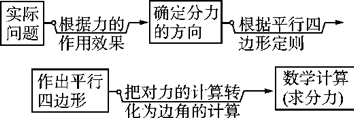
\includegraphics[width=0.5\textwidth]{521.png}
      \end{figure}

      如图所示,物体的重力G按产生的效果分解为两个分力,F1使物体下滑,F2使物体压紧斜面.
      \begin{figure}[htbp]
         \centering
         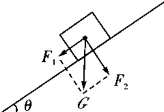
\includegraphics[width=0.2\textwidth]{522.png}
      \end{figure}

      \item 正交分解法
      \begin{itemize}
         \item 定义:将已知力按互相垂直的两个方向进行分解的方法.
         \item 建立坐标轴的原则:一般选共点力的作用点为原点,在静力学中,以少分解力和容易分解力为原则(使尽量多的力在坐标轴上);在动力学中,往往以加速度方向和垂直加速度方向为坐标轴建立坐标系.
         \item 方法:物体受到多个力F1、F2、F3……作用,求合力F时,可把各力向相互垂直的x轴、y轴分解.
         \begin{figure}[htbp]
            \centering
            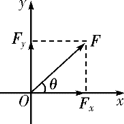
\includegraphics[width=0.1\textwidth]{523.png}
         \end{figure}
   
         \begin{itemize}
            \item x轴上的合力:Fx=Fx1+Fx2+Fx3+……
            \item y轴上的合力:Fy=Fy1+Fy2+Fy3+……
            \item 合力大小:F=F2x+F2y
            \item 合力方向:与x轴夹角为θ,则tan  θ=FyFx.

         \end{itemize}
      \end{itemize}
   \end{itemize}

   
   \begin{example}
      如图所示,光滑斜面的倾角为θ,有两个相同的小球,
      分别用光滑挡板A、B挡住,挡板A沿竖直方向,挡板B垂直于斜面,
      则两挡板受到小球压力的大小之比为,
      斜面受到两个小球压力大小之比为.      
      \begin{figure}[htbp]
         \centering
         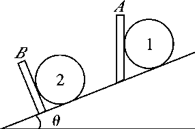
\includegraphics[width=0.2\textwidth]{524.png}
      \end{figure}

      \begin{solution}
         1∶cosθ;         1∶cos2θ
      \end{solution}

      
                  
      
   \end{example}

   \section{“绳——杆”模型}
   \begin{itemize}
      \item “死结”与“活结”模型
      \begin{itemize}
         \item “死结”可理解为把绳子分成两段,且不可以沿绳子移动的结点.
         “死结”两侧的绳因结而变成了两根独立的绳.
         \item “活结”可理解为把绳子分成两段,且可以沿绳子移动的结点.
         “活结”一般是由绳跨过滑轮或者绳上挂一光滑挂钩而形成的.实质还是同一根绳子.
      \end{itemize}
      \item “固定杆”与“活动杆”模型
      \begin{itemize}
         \item 一般情况下,插入墙中的杆属于固定杆(如钉子).
         \item 一端用铰链相连的杆属于活动杆.
      \end{itemize}
   \end{itemize}

   \begin{note}
      “绳——杆”模型的处理方法
      \begin{itemize}
         \item 无论“死结”还是“活结”一般均以结点为研究对象进行受力分析.
         \item 由“死结”分开的两段绳子上的弹力不一定相等;
         由“活结”分开的两段绳子上弹力的大小一定相等,
         两段绳子合力的方向一定沿这两段绳子夹角的平分线.
         \item 固定杆的弹力方向不一定沿杆的方向,而活动杆的弹力方向一定沿杆的方向.
      \end{itemize}   
   \end{note}

   \begin{example}
      如图甲所示,细绳AD跨过固定的水平轻杆BC右端的定滑轮挂住一个质量为M1的物体,
      ∠ACB=30°;图乙中轻杆HG一端用铰链固定在竖直墙上,
      另一端G通过细绳EG拉住,EG与水平方向也成30°,
      轻杆的G点用细绳GF拉住一个质量为M2的物体.求:

      \begin{figure}[htbp]
         \centering
         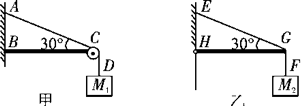
\includegraphics[width=0.3\textwidth]{531.png}
      \end{figure}
   
      \begin{solution}
      oa、ob为一根绳,两端拉力相等,设绳aob长为L,
      M、N的水平距离为d,bo延长线交M于a′,
      由几何知识知a′o=ao,sin θ=dL,
      由平衡条件有2Fcos θ=mg,则F=mg2cos θ,
      当b上移到b′时,d、L不变,θ不变,故F不变,
      选项A正确,C错误.将杆N向右移一些,L不变,d变大,θ变大,cos θ变小,
      则F变大,选项B正确.只改变m,其他条件不变,
      则sin θ不变,θ不变,衣架悬挂点不变,选项D错误. 
      \begin{figure}[htbp]
         \centering
         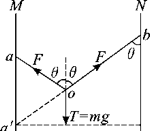
\includegraphics[width=0.3\textwidth]{514.png}
      \end{figure}
     
      \end{solution}
                  
      
   \end{example}

\chapter{受力分析共点力的平衡}
\begin{enumerate}
   \item 受力分析
   \begin{itemize}
      \item 定义:把指定物体(研究对象)在特定的物理环境中受到的所有外力都找出来,并画出受力图,这个过程就是受力分析.
      \item 受力分析的顺序:先找重力,再找接触力(弹力、摩擦力),最后分析电场力、磁场力及其他力.
      \item 受力分析的步骤
      \begin{itemize}
         \item 明确研究对象——确定分析受力的物体,研究对象可以是单个物体,也可以是多个物体的组合.
         \item 隔离物体分析——将研究对象从周围物体中隔离出来,进而分析物体受的重力、弹力、摩擦力、电磁力等,检查周围有哪些物体对它施加了力的作用
         \item 画出受力示意图——边分析边将力一一画在受力示意图上,准确标出方向
         \item 检查画出的每一个力能否找出它的施力物体,检查分析结果能否使研究对象处于题目所给的运动状态,否则,必然发生了漏力、添力或错力现象
         
      \end{itemize}
      
   \end{itemize}
   \item 共点力的平衡
   \begin{itemize}
      \item 平衡状态:物体处于静止或匀速直线运动状态
      \item 共点力的平衡条件:$F_{合}=0$或者$\left\{\begin{array}{l}{F_{x}=0} \\ {F_{y}=0}\end{array}\right.$
      \item 平衡条件的推论
      \begin{itemize}
         \item 二力平衡:如果物体在两个共点力的作用下处于平衡状态,这两个力必定大小相等、方向相反,为一对平衡力
         \item 三力平衡:如果物体在三个共点力的作用下处于平衡状态,其中任意两个力的合力一定与第三个力大小相等、方向相反
         \item 多力平衡:如果物体受多个力作用处于平衡状态,其中任何一个力与其余力的合力大小相等、方向相反
         
      \end{itemize}
   \begin{note}
      \begin{itemize}
         \item 物体在某一时刻速度为零时,物体不一定处于平衡状态
         \item 在多个共点力作用下的物体处于静止状态,如果其中一个力消失其他力保持不变,物体沿消失的力的反方向做初速度为零的匀加速直线运动
      \end{itemize}
      
   \end{note}
   \end{itemize}
   
\end{enumerate}

\section{对质点概念的理解}
\begin{enumerate}
   \item 
\end{enumerate}

\section{对质点概念的理解}
\begin{enumerate}
   \item 
\end{enumerate}

\section{对质点概念的理解}
\begin{enumerate}
   \item 
\end{enumerate}


\chapter{牛顿第一、第三定律}
\begin{enumerate}
   \item 牛顿第一定律
   \begin{itemize}
      \item 内容:一切物体总保持匀速直线运动状态或静止状态,直到有外力迫使它改变这种状态为止
      \item 意义
      \begin{itemize}
         \item 指出了一切物体具有惯性,因此牛顿第一定律又称惯性定律
         \item 指出力不是维持物体运动状态的原因,而是改变物体运动状态的原因,即力是产生加速度的原因
         \item 当物体不受力时,物体总保持匀速直线运动状态或静止状态
      \end{itemize}
      \item 惯性
      \begin{itemize}
         \item 定义:物体具有保持原来匀速直线运动状态或静止状态的性质
         \item 量度:质量是物体惯性大小的唯一量度,与物体的运动状态、受力情况、地理位置均无关,质量大的物体惯性大,质量小的物体惯性小
         \item 普遍性:惯性是物体的固有属性,一切物体都有惯性
      \end{itemize}
   \end{itemize}
   \item 牛顿第三定律
   \begin{itemize}
      \item 作用力和反作用力:两个物体之间的作用总是相互的,一个物体对另一个物体施加了力,另一个物体同时对这个物体也施加了力
      \item 内容:两个物体之间的作用力和反作用力总是大小相等、方向相反、作用在同一条直线上
      \item 表达式:$F=-F^{\prime}$
      \item 意义:建立了相互作用物体之间的联系及作用力与反作用力的相互依赖关系
   \end{itemize}
\end{enumerate}

\section{对质点概念的理解}
\begin{enumerate}
   \item 
\end{enumerate}

\section{对质点概念的理解}
\begin{enumerate}
   \item 
\end{enumerate}

\section{对质点概念的理解}
\begin{enumerate}
   \item 
\end{enumerate}


\chapter{牛顿第二定律两类动力学问题}
\begin{enumerate}
   \item 牛顿第二定律
   \begin{itemize}
      \item 内容:物体加速度的大小跟它受到的作用力成正比,跟它的质量成反比.加速度的方向与作用力的方向相同.
      \item 表达式:$F=m a$,$F$与$a$具有瞬时对应关系.
      \item 适用范围:
      \begin{itemize}
         \item 牛顿第二定律只适用于惯性参考系(相对地面静止或做匀速直线运动的参考系).
         \item 牛顿第二定律只适用于宏观物体(相对于分子、原子)、低速运动(远小于光速)的情况.
      \end{itemize}
   \end{itemize}
   \item 动力学两类基本问题
   \begin{itemize}
      \item 动力学两类基本问题
      \begin{itemize}
         \item 已知受力情况,求物体的运动情况
         \item 已知运动情况,求物体的受力情况
      \end{itemize}
      \item 解决两类基本问题的方法:以加速度为“桥梁”,由运动学公式和牛顿运动定律列方程求解,具体逻辑关系如图所示.
   \end{itemize}
\end{enumerate}

\section{对质点概念的理解}
\begin{enumerate}
   \item 
\end{enumerate}

\section{对质点概念的理解}
\begin{enumerate}
   \item 
\end{enumerate}

\section{对质点概念的理解}
\begin{enumerate}
   \item 
\end{enumerate}


\chapter{牛顿运动定律的综合应用}
\begin{enumerate}
   \item 超重和失重
   \begin{itemize}
      \item 实重与视重
      \begin{itemize}
         \item 实重:物体实际所受的重力,与物体的运动状态无关
         \item 视重:当物体挂在弹簧测力计下或放在水平台秤上时,弹簧测力计或台秤的示数称为视重;视重大小等于弹簧测力计所受物体的拉力或台秤所受物体的压力
      \end{itemize}
      \item 超重、失重和完全失重的比较
      
   \end{itemize}
   \item 连接体问题
   \begin{itemize}
      \item 整体法和隔离法
      \begin{itemize}
         \item 整体法:当连接体内(即系统内)各物体的加速度相同时,可以把系统内的所有物体看成一个整体,分析其受力和运动情况,运用牛顿第二定律对整体列方程求解的方法.
         \item 隔离法:当求系统内物体间相互作用的内力时,常把某个物体从系统中隔离出来,分析其受力和运动情况,再用牛顿第二定律对隔离出来的物体列方程求解的方法.
      \end{itemize}
      \item 动力学图象
      \begin{itemize}
         \item 三种图象:v-t图象、a-t图象、F-t图象
         \item 图象间的联系:加速度是联系v-t图象与F-t图象的桥梁
      \end{itemize}
   \end{itemize}
\end{enumerate}

\section{对质点概念的理解}
\begin{enumerate}
   \item 
\end{enumerate}

\section{对质点概念的理解}
\begin{enumerate}
   \item 
\end{enumerate}

\section{对质点概念的理解}
\begin{enumerate}
   \item 
\end{enumerate}


\chapter{曲线运动 运动的合成与分解}
\begin{enumerate}
   \item 
\end{enumerate}

\section{对质点概念的理解}
\begin{enumerate}
   \item 
\end{enumerate}

\section{对质点概念的理解}
\begin{enumerate}
   \item 
\end{enumerate}

\section{对质点概念的理解}
\begin{enumerate}
   \item 
\end{enumerate}


\chapter{抛体运动的规律及应用}
\begin{enumerate}
   \item 
\end{enumerate}

\section{对质点概念的理解}
\begin{enumerate}
   \item 
\end{enumerate}

\section{对质点概念的理解}
\begin{enumerate}
   \item 
\end{enumerate}

\section{对质点概念的理解}
\begin{enumerate}
   \item 
\end{enumerate}


\chapter{圆周运动的规律及应用}
\begin{enumerate}
   \item 
\end{enumerate}

\section{对质点概念的理解}
\begin{enumerate}
   \item 
\end{enumerate}

\section{对质点概念的理解}
\begin{enumerate}
   \item 
\end{enumerate}

\section{对质点概念的理解}
\begin{enumerate}
   \item 
\end{enumerate}


\chapter{万有引力与航天}
\begin{enumerate}
   \item 
\end{enumerate}

\section{对质点概念的理解}
\begin{enumerate}
   \item 
\end{enumerate}

\section{对质点概念的理解}
\begin{enumerate}
   \item 
\end{enumerate}

\section{对质点概念的理解}
\begin{enumerate}
   \item 
\end{enumerate}


\chapter{功和功率}
\begin{enumerate}
   \item 
\end{enumerate}

\section{对质点概念的理解}
\begin{enumerate}
   \item 
\end{enumerate}

\section{对质点概念的理解}
\begin{enumerate}
   \item 
\end{enumerate}

\section{对质点概念的理解}
\begin{enumerate}
   \item 
\end{enumerate}


\chapter{动能定理及其应用}
\begin{enumerate}
   \item 
\end{enumerate}

\section{对质点概念的理解}
\begin{enumerate}
   \item 
\end{enumerate}

\section{对质点概念的理解}
\begin{enumerate}
   \item 
\end{enumerate}

\section{对质点概念的理解}
\begin{enumerate}
   \item 
\end{enumerate}


\chapter{机械能守恒定律及其应用}
\begin{enumerate}
   \item 
\end{enumerate}

\section{对质点概念的理解}
\begin{enumerate}
   \item 
\end{enumerate}

\section{对质点概念的理解}
\begin{enumerate}
   \item 
\end{enumerate}

\section{对质点概念的理解}
\begin{enumerate}
   \item 
\end{enumerate}


\chapter{功能关系能量守恒定律}
\begin{enumerate}
   \item 
\end{enumerate}

\section{对质点概念的理解}
\begin{enumerate}
   \item 
\end{enumerate}

\section{对质点概念的理解}
\begin{enumerate}
   \item 
\end{enumerate}

\section{对质点概念的理解}
\begin{enumerate}
   \item 
\end{enumerate}


\chapter{运动的描述 匀变速直线运动的研究}
%======================================================

\nocite{*} 

\bibliography{reference}

\appendix
\chapter{物理学史}

本附录包括了

\begin{equation}
\sum_{i=1}^n x_i \equiv x_1 + x_2 +\cdots + x_n
\end{equation}



\chapter{公式图表}



\end{document}
